% !TEX encoding = UTF-8 Unicode
% \documentclass{article}
% \usepackage{../../superstyle}
% \usepackage{listings}
% \usepackage{amsmath}
% \begin{document}
% remove all before

%oppgavetekst
If the Matlab Symbolic Toolbox is available (or a symbolic package such as Maple
or Mathematica), an alternative to Step 2 is possible. Define symbolic variables by using the syms command and solve the simultaneous equations with the Symbolic Toolbox command solve. Use subs to evaluate the symbolic result as a floating point number.

\vspace{5mm}

Løsning


\begin{lstlisting}[caption={Task3.m}]
function [ test, ans ] = task3()

A1 = 15600;
B1 = 7540;
C1 = 20140;
t1 = 0.07074;

A2 = 18760;
B2 = 2750;
C2 = 18610;
t2 = 0.07220;

A3 = 17610;
B3 = 14630;
C3 = 13480;
t3 = 0.07690;

A4 = 19170;
B4 = 610;
C4 = 18390;
t4 = 0.07242;

c = 299792.458;

syms x y z d;

f = [(x-A1).^2 + (y-B1).^2 + (z-C1).^2 - (c.*(t1-d)).^2 == 0,
    (x-A2).^2 + (y-B2).^2 + (z-C2).^2 - (c.*(t2-d)).^2 == 0, 
    (x-A3).^2 + (y-B3).^2 + (z-C3).^2 - (c.*(t3-d)).^2 == 0, 
    (x-A4).^2 + (y-B4).^2 + (z-C4).^2 - (c.*(t4-d)).^2 == 0];

S = solve(f, x, y, z, d);

% sjekker at likningen går opp
test = isAlways(subs(f, S));

% lager en matrise av x, y og z koordinatene + d
Sv = [S.x, S.y, S.z, S.d];

% henter ut koordinatene der z ligger nermest jordradiusen
riktig_pos = 2;
if (abs(S.z(1) - 6371) < abs(S.z(2) - 6371)) riktig_pos = 1; end
ans = eval(Sv(riktig_pos,[1:length(Sv)]));

end
\end{lstlisting}

\begin{figure}[h]
    \centering
    \includegraphics[width=1\textwidth]{sections/Exercise6/task3result}
    % \includegraphics[width=1\textwidth]{task3result}
    \caption{Task 3 - resultat}
    \label{fig:task3result}
\end{figure}

Som vi ser ut fra figur \ref{fig:task3result} blir svarene tilnermet det samme som når vi regnet det ut manuelt i oppgave 2.

% remove after
% \end{document}